\documentclass{article}
\usepackage{graphicx} % new way of doing eps files
\usepackage{listings} % nice code layout
\usepackage[usenames]{color} % color
\definecolor{listinggray}{gray}{0.9}
\definecolor{graphgray}{gray}{0.7}
\definecolor{ans}{rgb}{1,0,0}
\definecolor{blue}{rgb}{0,0,1}
% \Verilog{title}{label}{file}
\newcommand{\Verilog}[3]{
  \lstset{language=Verilog}
  \lstset{backgroundcolor=\color{listinggray},rulecolor=\color{blue}}
  \lstset{linewidth=\textwidth}
  \lstset{commentstyle=\textit, stringstyle=\upshape,showspaces=false}
  \lstset{frame=tb}
  \lstinputlisting[caption={#1},label={#2}]{#3}
}


\author{Matthew Carrano and Breana Leal}
\title{Lab 3 - Fetch Stage}

\begin{document}
\maketitle

\section{Introduction}
The goal of this lab is to create an instruction memory module and combine previous modules to form the fetch stage, iFetch.  The instruction memory  will be used to store instructions. The instruction memory reads in data from the program counter that requires addressing executable instructions. The fetch stage is the first stage in building the ARM computer that combines the previous labs. The fetch stage will be followed by the decode stage.
  
\section{Interface}
The inputs of the instruction memory module are clk and pc. The clk is initiated to follow a positive clock edge. With each cycle, pc will increment which should give a value for its output instruction to address from a memory file.  
The inputs of the iFetch are clk, reset, pc\_src, and branch\_target. The output of the iFetch is incremented\_pc, instruction, and cur\_pc. Its inputs and outputs serve as connecting pieces for the previously discussed modules mux, register, adder, and instruction memory.

incremented\_pc and branch\_target are the two signals that are available to be selected, and pc\_src is the signal that is used to select whether the value of incremented\_pc or branch\_target will be chosen by the mux. new\_pc is a wire that contains the value that the mux selected. The output from the mux becomes an input for the register along with inputs clk and reset. The output for the register becomes cur\_pc. Similarly, cur\_pc becomes an input for the adder module. The adder's other input is STEP, a parameter defined as 'WORD'd4 and its output is incremented\_pc. Finally, the instru\_mem module has inputs clk and cur\_pc. The cur\_pc is the current program counter value and notifies ARM about the current instruction address. The output instruction is the final data from the provided memory file. 

As noted, the fetch stage connects the previous modules in having one's input become another's output and reiterate the process to continuously update the instruction results either sequentially or branching.
\section{Design}
The first module to build is the instruction memory module.  The instruction memory module is designed to take one 64-bit input value and produce a 32-bit data from a readable file as an output.

The second module to build is the iFetch module.  The iFetch module is designed to process five input values with four individually instantiated modules (discussed in Interface). Each module processes its own inputs to has its own output that work under the iFetch module to evaluate the final instruction value for the fetch stage to pass onto the decode stage. 
\section{Implementation}
The instruction memory module is implemented by having a 32-bit data reg imem. The output instruction is set to equal the program counter divided by 4 indexed data. Meaning, the instruction should equal the adjusted 32 bit data read from the file. For example, if the program counter is set to 8, the instruction will out put the binary code, line 2, from the readable file. This is done continuously and updated with each input change.
\Verilog{Verilog code for implementing the instruction memory.}{code:adder}{../code/1_fetch/instr_mem.v}

The iFetch module is implemented instantiating the mux, register, adder, and instruction memory modules. The instantiations easily verify the connections the fetch stage makes. 

mux is altered to have a WORD parameter and instruction memory SIZE parameter for future reference purposes. 
\Verilog{Verilog code for implementing the Fetch Stage.}{code:mux}{../code/1_fetch/iFetch.v}

\section{Test Bench Design}
The adder test bench creates regs for a and b as well as a wire for the add\_out output of the adder module.  All signals are 64-bits.  An adder module, UUT, is instantiated, and then a series of a and b inputs are set in the initial section.  Regs a and b are set using non-blocking procedural assignments, then a cycle delay is initiated.  As defined in definitions.vh, a cycle is 10ns.  Then a and b are changed several times, with various amounts of delay.  The goal is to test a variety of inputs and outputs at various intervals.  The results of the test are verified by evaluating the simulation results and verifying that add\_out equals a + b at all times.  View the adder\_test code in Listing~\ref{code:addertest} on page~\pageref{code:addertest}.

\Verilog{Verilog code for testing the Instruction Memory.}{code:addertest}{../code/1_fetch/instr_mem_test.v}


The mux test bench creates regs for a, b, and control as well as a wire for the mux\_out output of the mux module.  All signals are 64-bits.  An adder module, UUT, is instantiated with a size of 64 by using the syntax of mux\#(64) UUT.  Then a series of a and b inputs are set in the initial section, and the control line is set to 0.  a and b are varied with various amounts of delay.  After several cycles, control is changed to 1, causing the value of b to be sent to mux\_out.  And then control is set back to 0 to verify that the mux can switch back and forth effectively.  The results of the test are verified by evaluating the simulation results and verifying that:
\begin{enumerate}
	\item mux\_out always equals a when control is 0 
	\item mux\_out always equals b when control is 1
\end{enumerate} 
View the mux\_test code in Listing~\ref{code:muxtest} on page~\pageref{code:muxtest}.

\Verilog{Verilog code for testing the Fetch Stage.}{code:muxtest}{../code/1_fetch/iFetch_test.v}

\section{Simulation}
The Simulation Results of the adder test confirm that the adder works as expected, with add\_out always producing the sum of a and b.  The timing diagram can be viewed in Figure~\ref{fig:addertest} on page~\pageref{fig:addertest}.

The Simulation Results of the mux test confirm that the mux works as expected, with mux\_out always matching the conditions listed in the Test Bench Design section.  The timing diagram can be viewed in Figure~\ref{fig:muxtest} on page~\pageref{fig:muxtest}.

\begin{figure}
\begin{center}
\caption{Timing diagram for the instruction memory test (First Half).}\label{fig:addertest}
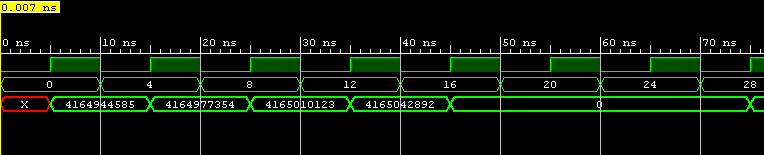
\includegraphics[width=0.9\textwidth]{../images/instr_memSim1.png}
\end{center}
\end{figure}

\begin{figure}
	\begin{center}
		\caption{Timing diagram for the instruction memory (Second Half) test.}\label{fig:muxtest}
		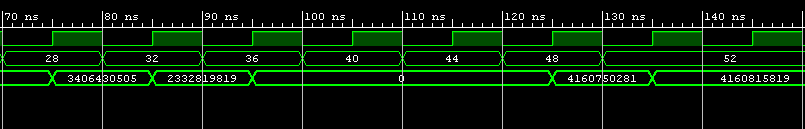
\includegraphics[width=0.9\textwidth]{../images/instr_memSim2.png}
	\end{center}
\end{figure}

\section{Conclusions}
The instruction module and fetch stage were successfully established.  The instruction memory module is used in conjunction with the mux, register, and adder modules. The instruction memory is established to gather data from a file based on addressed instruction values from the program counter. Combined, these modules form the first stage for the ARM-64 that will be further processes in the decoding stage.

\end{document} 